\providecommand{\main}{..}
\documentclass[\main/main.tex]{subfiles}
\begin{document}

\chapter{Giochi simmetrici}

\begin{definition}[Gioco simmetrico]
  Un gioco è \textbf{simmetrico} quando tutti i giocatori hanno lo stesso numero di strategie pure e per ogni permutazione delle strategie (se i giocatori scambiano strategia) si permutano allo stesso modo i payoff risultanti.
\end{definition}

\begin{definition}[Gioco simmetrico a due persone]
  In un gioco simmetrico a due persone, la matrice dei guadagni del secondo giocatore è la trasposta della matrice dei guadagni del primo giocatore.
\end{definition}

\section{Tassonomia dei giochi simmetrici a due persone e due strategie}
\subsection{Matrimonio perfetto}
\[
  f_{11} > f_{21} > f_{12} > f_{22}
\]

\begin{figure}
  \begin{subfigure}{0.49\textwidth}
    
\includegraphics[width=0.7\textwidth]{marriage}
  \end{subfigure}
  \begin{subfigure}{0.49\textwidth}
    \begin{table}
      \begin{tabular}{|L|L|L|}
        \hline
           & C                      & NC             \\
        \hline
        C  & (\tilde{3}, \tilde{3}) & (\tilde{1}, 2) \\
        \hline
        NC & (2, \tilde{1})         & (0,0)          \\
        \hline
      \end{tabular}
    \end{table}
  \end{subfigure}
  \caption{Gioco del matrimonio perfetto}
\end{figure}

\begin{description}
  \item[C] Il coniuge collabora.
  \item[NC] Il coniuge non collabora.
\end{description}

Quando entrambi collaborano si ha il payoff massimo, ma anche quando uno non collabora e il secondo si, per quando si trovi in una situazione non preferibile è comunque migliore che non collaborare entrambi.

\subsection{Caccia al cervo}
\[
  f_{11} > f_{21} > f_{22} > f_{12}
\]

\begin{figure}
  \begin{subfigure}{0.49\textwidth}
    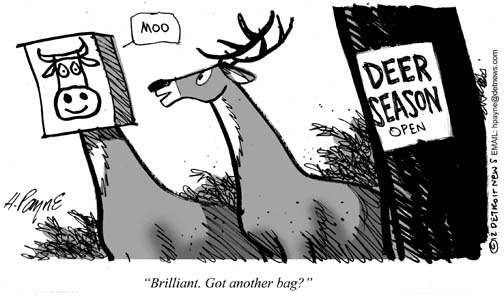
\includegraphics[width=0.7\textwidth]{deer}
  \end{subfigure}
  \begin{subfigure}{0.49\textwidth}
    \begin{table}
      \begin{tabular}{|L|L|L|}
        \hline
           & C                      & NC                    \\
        \hline
        C  & (\tilde{3}, \tilde{3}) & (0, 2)                \\
        \hline
        NC & (2, 0)                 & (\tilde{1},\tilde{1}) \\
        \hline
      \end{tabular}
    \end{table}
  \end{subfigure}
  \caption{Gioco della caccia al cervo}
\end{figure}

\begin{description}
  \item[C] Il cacciatore collabora.
  \item[NC] Il cacciatore non collabora.
\end{description}

Se i due cacciatori collaborano probabilmente catturano il cervo, se uno non collabora e l'altro cerca di collaborare probabilmente quello che non collabora riesce a catturare una preda minore (es. lepre) mentre se entrambi non collaborano forse possono catturare ognuno una preda minore.

\section{Giochi di coordinamento puro}
\subsection{Gioco del coniglio}

\[
  f_{21} > f_{11} > f_{12} > f_{22}
\]

\begin{figure}
  \begin{subfigure}{0.49\textwidth}
    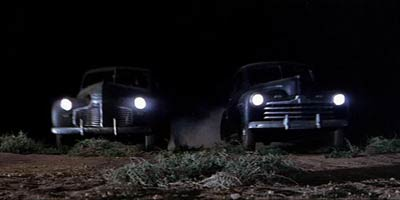
\includegraphics[width=0.7\textwidth]{chicken}
  \end{subfigure}
  \begin{subfigure}{0.49\textwidth}
    \begin{table}
      \begin{tabular}{|L|L|L|}
        \hline
           & C                      & NC                     \\
        \hline
        C  & (2, 2)                 & (\tilde{1}, \tilde{3}) \\
        \hline
        NC & (\tilde{3}, \tilde{1}) & (0,0)                  \\
        \hline
      \end{tabular}
    \end{table}
  \end{subfigure}
  \caption{Corsa del coniglio}
\end{figure}

\begin{description}
  \item[C] Il pilota frena.
  \item[NC] Il pilota non frena.
\end{description}

Nella corsa del coniglio due piloti si sfidano a chi frenerà per ultimo prima di un precipizio. Se uno dei due frena l'altro vince ed entrambi rimangono vivi. Se entrambi frenano, nessuno vince ma rimandono vivi. Se nessuno dei due frena si schiantano.

\subsection{La guerra dei sessi}

\[
  f_{12}>f_{21}>f_{22}>f_{11} \land f_{21}>f_{12}>f_{22}>f_{11}
\]

\begin{figure}
  \begin{subfigure}{0.49\textwidth}
    
\includegraphics[width=0.7\textwidth]{sessi}
  \end{subfigure}
  \begin{subfigure}{0.49\textwidth}
    \begin{table}
      \begin{tabular}{|L|L|L|}
        \hline
           & C                      & NC                     \\
        \hline
        C  & (0, 0)                 & (\tilde{2}, \tilde{3}) \\
        \hline
        NC & (\tilde{3}, \tilde{2}) & (1,1)                  \\
        \hline
      \end{tabular}
    \end{table}
  \end{subfigure}
  \caption{La guerra dei sessi}
\end{figure}

\begin{description}
  \item[C] L'innamorato decide di seguire il piano dell'altro.
  \item[NC] L'innamorato decide di seguire il proprio piano.
\end{description}

Due innamorati litigano al telefono su che piano seguire per la serata. Cade la linea e devono decidere che cosa fare, considerando che andare da soli rimanda sgradevole.

Se ognuno segue il piano stabilito dall'altro ognuno segue da solo qualcosa che non vuole. Se ognuno non collabora, ognuno segue qualcosa che vuole da solo. Se uno solo dei due collabora, segue qualcosa che non vuole ma almeno lo fa in compagnia.

\subsection{Il dilemma del prigioniero}

\[
  f_{21}>f_{11}>f_{22}>f_{12}
\]

\begin{figure}
  \begin{subfigure}{0.49\textwidth}
    
\includegraphics[width=0.7\textwidth]{prisoner}
  \end{subfigure}
  \begin{subfigure}{0.49\textwidth}
    \begin{table}
      \begin{tabular}{|L|L|L|}
        \hline
           & C              & NC                    \\
        \hline
        C  & (2, 2)         & (0, \tilde{3})        \\
        \hline
        NC & (\tilde{3}, 0) & (\tilde{1},\tilde{1}) \\
        \hline
      \end{tabular}
    \end{table}
  \end{subfigure}
  \caption{La guerra dei sessi}
\end{figure}

\begin{description}
  \item[C] Il prigioniero non tradisce l'altro arrestato.
  \item[NC] Il prigioniero tradisce l'altro arrestato.
\end{description}

Due persone vengono arrestato con prove sufficienti per incriminare almeno uno e l'altro per collaborazione. I poliziotti sanno chi dei due sia effettivamente più colpevole.

Se un prigioniero parla e l'altro tace prende uno sconto sulla pena e l'altro la pena massima. Se entrambi tacciono nessuno prende la pena massima ma nemmeno lo sconto. Se entrambi parlano avranno entrambi la pena massima.

\end{document}